\section{Kesimpulan}

Pengerjaan Tugas Besar 1 ini menunjukkan bahwa pendekatan greedy dapat diimplementasikan secara efektif pada permainan Battlecode 2025 melalui perancangan fungsi seleksi lokal, fungsi kelayakan, dan fungsi objektif yang konsisten dengan peran tiap unit (Soldier, Splasher, Mopper, dan Tower). Dari rangkaian implementasi, eksperimen, dan evaluasi pertandingan, strategi yang menonjol adalah greedy based on scoring atau nearest target karena mampu menjaga tekanan serangan terhadap tower lawan sekaligus mempertahankan keberlanjutan sumber daya melalui mekanisme refill, koordinasi pesan, serta navigasi yang baik. Secara keseluruhan, hasil pengujian memperlihatkan bahwa kualitas heuristik lokal sangat menentukan performa akhir bot, dan kombinasi keputusan yang sederhana namun cepat dieksekusi memberikan keunggulan pada lingkungan permainan yang dinamis.

\section{Saran}

Selanjutnya, kelompok kami menyarankan agar pengembangan bot ini membuatnya semakin adapatif agar keputusan dapat diambil secara otomatis sesuai fase permainan, tipe peta, dan gaya lawan. Selain itu, kualitas evaluasi dapat ditingkatkan dengan eksperimen yang lebih sistematis sehingga perbandingan antar strategi menjadi lebih objektif. Dengan waktu yang singkat dalam megerjakan tugas besar ini, kelompok kami yakin bahwa ada heuristik yang lebih baik lagi jika kita mengoptimisasi heuristik yang telah disampaikan pada laporan ini. Oleh karena itu, pengujian dengan berbagai macam robot yang telah diciptakan untuk kontes ini sangat dibutuhkan dalam memberikan pemahaman baru kepada kelompok kami.

\vspace{5cm}

Tugas ini disusun sepenuhnya tanpa bantuan kecerdasan buatan (\textit{Generative AI}),
melainkan hasil pemikiran dan analisis mandiri.
\begin{flushright}
    
\includegraphics[width=4cm]{public/sign_kevin.jpg}\\
    Kevin Wirya Valerian [13524019]
\end{flushright}

\begin{flushright}
    
\includegraphics[width=6cm]{public/sign_aufar.png}\\
    Muhammad Aufar Rizqi Kusuma [13524061]
\end{flushright}

\begin{flushright}
    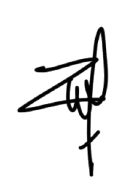
\includegraphics[width=6cm]{public/sign_athilla.png}\\
    Muhammad Aufar Rizqi Kusuma [13524061]
\end{flushright}